\section{Multivariable Linear Regression}
A linear regression model for 2 features:
\begin{align*}
  a(x_1, x_2) &= w_1\,x_1 + w_2\,x_2 + b \\
   &= \vec{w}\cdot\vec{x} + b
\end{align*}
$w_1$,$w_2$ control the slopes of this plane, $b$ translates it up and down. $\vec{x}$ is for one sample. Two or more samples are represented as a matrix:
\begin{align*}
[a_1, a_2] = 
  [w_1, w_2]\cdot{}
  \begin{bmatrix}
  x_1 & x_1\\
  x_2 & x_2 
  \end{bmatrix}
 +  b
\end{align*}
$a_i$ is the result for each sample (columns in the matrix).

The same than for a line (figure \ref{fig:line}) by tuning $W$ and $b$  we can find the best linear fit. The sign of $W$ reflects the line over Y($a$) axis, and its magnitude controls the slope; $b$ translates the line over $x$. Without $b$ the line has to go through the origin. 

We need to do forward and backward propagation.
\begin{figure}[h]
 \centering
 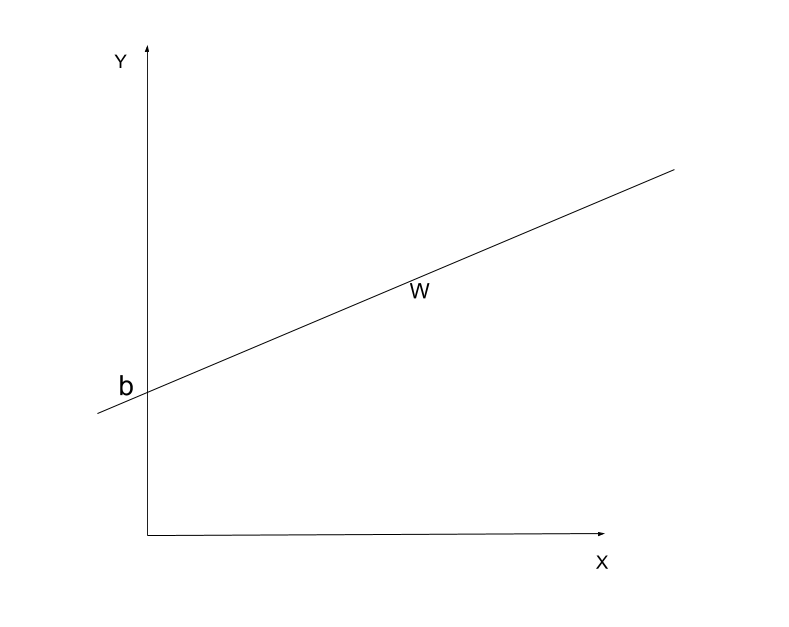
\includegraphics[width=0.9\textwidth]{line_plot.png}
  \caption{Line plot} \label{fig:line}
\end{figure}


\subsection{Forward Propagation}
A general network scheme is shown in \ref{fig:single}. Calculations are built following that network scheme. 
\begin{itemize}
  \item The activation is a linear function:
    \[ \hat{\vec{a}} = \vec{w}\cdot\mathbf{X} + \vec{b}\]
  \item The Loss $= Loss(w_1,\ldots, w_n, b)$ or just $L(\vec{w},b)$ is the \textit{Square Error}:
  \[
  L_i(\vec{w}, b) = (a_i - \hat{a})^2\\
  =(a_i -\sum_j\,w_j\mathbf{X}_{ji} -b)^2
\]
$\sum_j w_j\,\mathbf{X}_{ji}$ is the dot product.

\item The cost is the averaged sum of $L_i$, and it's the \textit{Mean Square Error}:
\begin{align}
  C(w_1, w_2, b) &= \frac{1}{2} \sum_{i=0}^{i=2} L_i(w_1, w_2, b)\nonumber\\
  &= \frac{1}{2}([a_1, a_2] - [\hat{a}_1, \hat{a}_2])\cdot{}([a_1, a_2]-[\hat{a}_1, \hat{a}_2])\nonumber\\
  &=\frac{1}{2}([a_1, a_2] - [w_1, w_2]\cdot{}\mathbf{X}-b)\cdot{}([a_1, a_2] - [w_1,w_2]\cdot{}\mathbf{X} -b) \label{cost}
\end{align}
$\frac{1}{2}$ is to average over samples. Equation \ref{cost} is what we implement into code.
%Outliers may be critical on the effect of weights and biases.
\end{itemize}
In Python it'd look like:
\begin{center}
  \begin{BVerbatim}
  Ap = np.dot(w,X) - b
  diff = A-Ap 
  cost = 1/2*np.dot(diff, diff.T)
  \end{BVerbatim}
\end{center}





\subsection{Backward Propagation}
\begin{figure}
  \centering
  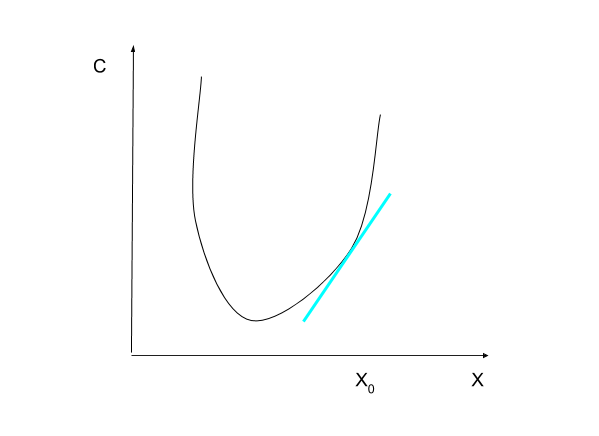
\includegraphics[width=0.75\textwidth]{derivative.png}
  \caption{Derivative}\label{fig:basics}
\end{figure}

For a function of a single variable $C(x)$ the derivative at a point $x_0$ is the slope (figure \ref{fig:basics}) at $x_0$.

For many variables, it's a similar process: the total derivative of a function is the sum of partial derivatives.

\begin{align}
  dC(\vec{w},b) &= \frac{\partial C}{\partial w_1}+ \frac{\partial C}{\partial w_2} + \frac{\partial C}{\partial b}\\
\end{align}
$C(w,b)$ derivative is used to find better weights and bias:
\begin{align*}
  \vec{w} &= [w_1, w_2] - [\frac{\partial C}{\partial w_1},\frac{\partial C}{\partial w_2}]\cdot{}\alpha\\
  \vec{w} &= \vec{w} -\frac{\partial C}{\partial \vec{w}}\cdot{}\alpha\\
  b &= b -\frac{\partial C}{\partial b}\cdot{}\alpha
\end{align*}
Let's get started.
\begin{align}
  dC(\vec{w},b) &= \frac{\partial C}{\partial w_1}+ \frac{\partial C}{\partial w_2} + \frac{\partial C}{\partial b}\label{eq:start}\\
  &= d(\sum_{i=0}^{i=2}L_i) = \sum_{i=0}^{i=2}dL_i(\vec{w},b) \label{diffp}\\
  &=\sum_{i=0}^{i=2} \frac{\partial L_i}{\partial w_1} +\frac{\partial L_i}{\partial w_2} + \frac{\partial L}{\partial b}\nonumber
\end{align} 
These equations are important. Equation \ref{eq:start} is always the starting point in any method. Equation \ref{diffp} makes use of linearity property of diff.

What we look for is:
\begin{align}
  \frac{\partial C}{\partial w_1} &= c\sum_i \frac{\partial L_i}{\partial w_1} = c\sum_i \frac{\partial L_i}{\partial A_i}\frac{A_i}{\partial w_1}\nonumber\\
  &\vdots\nonumber\\
  \frac{\partial C}{\partial w_n} &= c\sum_i \frac{\partial L_i}{\partial w_n}  = c\sum_i \frac{\partial L_i}{\partial A_i}\frac{A_i}{\partial w_n} \label{eq:cost_vector} 
\end{align}
(Remember, updating $w$, $b$, minimizing $C$, fits line to data. That's why we are deriving). Last equality uses the chain rule $df(g(x)) = \frac{df}{dg}\frac{dg}{dx}$. 

\begin{align*}
  L_k(\vec{w},b) &= (a_k - \hat{a}_k)^2
\end{align*}
$A_k$ is the difference $a_k-\hat{a}_k$. We need $dw$ and $db$; and for this $dA_k$:

\begin{align*}
  \frac{\partial L_k}{\partial w_j} &= 2A_k\,\frac{\partial(a_k - w_j\,\mathbf{X}_{jk} - b)}{\partial w_j}\\
\sum_k \frac{\partial L_k}{\partial w_j} &= -2\sum_k A_k\,\mathbf{X}_{jk}\\
\end{align*}
Replacing results in equations \ref{eq:cost_vector}. For example: 
\begin{align*}
  \frac{\partial C}{\partial w_1} &= \frac{1}{2}\, 2\sum_i \mathbf{X}_{1i}\,(a_i-\hat{a}_i) \\
  &= \frac{1}{2}\, 2\sum_i \mathbf{X}_{1i}\,A_i 
\end{align*}

Finally, using \textit{Gradient Descent} method, we update vectors:

\begin{align}
  \vec{w} &= \vec{w} -\frac{\partial C}{\partial \vec{w}}\,\alpha\nonumber\\
  &= \vec{w} +\frac{1}{2}\times{}2\mathbf{X}\cdot{}\vec{A^T}\,\alpha\\ 
  b &= b -\frac{\partial C}{\partial b}\cdot{}\alpha\nonumber\\
  &= b +\frac{1}{2}\times{}2\vec{A}\times{}\vec{1}\,\alpha
\end{align}
$\alpha$ is called \textit{learning rate} and we use to tune the derivation. We go against the gradient so the sign is changed to $-$ (it points to max increasing direction otherwise).

\subsubsection{Interpretation}

There is no graphical justification as to why we update $w$ and $b$ like that, but we are moving $w$ against (minus) the gradient multiplied by a constant (alpha) called \textit{learning rate}.

The minus sign is because the gradient always points away from the minimum and we want towards it (in one dimension there are only 2 directions). 

\begin{align}
  \vec{w} &= \vec{w} -\frac{\partial C}{\partial \vec{w}}\,\alpha\\
  &= \vec{w} -\left[\frac{\partial C}{\partial w_1}, \frac{\partial C}{\partial w_2},\ldots, \frac{\partial C}{\partial w_n}\right]\,\alpha
\end{align}

It means we have a vector of corrections for each slope such that the overall cost is decreased. If we take say $\frac{dC}{dw_1}$ it is the sum of slopes for each sample, divided by $m$. 

The slope depends on the sum of features times errors, as it was found: 
\begin{align*}
  \frac{\partial C}{dw_1}&= -\frac{2}{m}\sum_i \mathbf{X}_{1i}(\vec{a}_i-\vec{\hat{a}}_i)
\end{align*}

%This is almost the same result we get in the \textit{sigmoid}, just multiplied by $2$. Because the $2$ can be thought as inside the learning rate, we can use the exact same \textit{backpropagation} for both methods!

\subsection{Many features and samples}
For a larger problem, the only difference is the size of the matrices.

The problem is to find $w_i$, $b$ such that the multidimensional ``plane'' has small error respect to each datapoint. Then for a new datapoint we will have a trained predictor.

As it was shown, for linear regression the model is:
\begin{align*}
  \hat{a}(\vec{x}) &= w_1\,x_1 + w_2\,x_2 +\ldots+ w_n\,x_n\\
   &= \sum_i^n w_i\, x_i + b \\
   &= \vec{w}\cdot\vec{x} + b
\end{align*}
Here $\vec{x}$ is for one sample. For $n$ samples, it becomes a matrix, we write $\hat{\vec{a}} = \vec{w}\cdot\mathbf{X} + \vec{b}$. This is represented:
\begin{equation*}
  [a_1, a_2, \ldots, a_n] = 
  [w_1, w_2, \ldots, w_n] \cdot
  \begin{bmatrix}
    x_{11} & x_{12} & \ldots & x_{1m}\\
    x_{21} & x_{22} & \ldots & x_{2m}\\
    \vdots & \vdots & \ddots & \vdots\\
    x_{n1} & x_{22} & \ldots & x_{nm}\\
  \end{bmatrix}
  + [b_1, b_2, \ldots, b_m]
\end{equation*}
The $b_i$ are all the same number. There are $m$ examples-columns with $n$ features-rows. Hence $[\mathbf{X}] = m\times{}n$

The results are exactly the same than the previous section.
